\chapter{Developing a cross-domain Reddit dataset} \label{chap:reddit-data}

In order to explore transfer learning between the domains of news articles and social media comments for the task of political bias detection, we create a novel cross-domain dataset containing a set of news articles that have been shared on Reddit, and the accompanying Reddit comments, both annotated by political bias. We create our own such dataset since, as mentioned in Section \ref{subsec:collecting-reddit-data}, no pre-existing datasets of this type exist in the literature.

In this chapter we discuss the challenges faced in creating a high-quality dataset, and the data sources we consider. News articles and Reddit comments present different (but related) domains of text that can be explored and compared - in this chapter we also examine similarities between the different domains in our dataset.

We mentioned in Section \ref{subsec:domain-adaptation} that unsupervised domain adaptation methods do not need labelled data in the target domain, so we could theoretically explore transfer learning from news articles to social media comments without needing annotated comments. However, in order to evaluate performance of these domain adaptation methods with metrics such as F1 and accuracy, comments with labels are inevitably needed. Hence, in our dataset both news articles and Reddit comments are annotated by political bias.

\section{Designing a high-quality dataset}

Here we look at several issues faced in creating a high-quality dataset.

\subsection{Finding suitable annotations} \label{subsec:annotations}

One major design decision we face is how to find suitable annotations for Reddit comments, since this influences later decisions on where (and how) to source our data.

Typically, posts and comments on social media are not annotated with political leaning, perhaps explaining why the task of exploring political bias on this medium is such a challenging one. However, we can exploit one of the unique features of Reddit, that of subreddits. Posts and comments on Reddit are naturally grouped into communities, and a wide range of popular and politically-related subreddits are available to browse on Reddit, such as r/liberal, r/conservative, r/republican, etc. These subreddit titles provide natural political-bias annotations for the content displayed within each of those subreddits.

One key assumption to examine here is that all content under a particular subreddit will necessarily follow that particular political leaning. For example, whereas most comments in r/liberal may be from subscribers to that subreddit, nothing stops members of another subreddit such as r/conservative from leaving comments under r/liberal and starting a discussion.

However, it has been shown that this occurs very infrequently. A study by Guimaraes et al. \cite{guimaraes} quantified and examined cases of \textit{harmony} and \textit{dispute} among Reddit posts, where \textit{dispute} is defined as a comment thread where one particular set of comments attracts a notable amount of downvotes from the community, and \textit{harmony} is a comment thread where no such set of downvoted comments exists. They find that in two major political subreddits (r/politics and r/worldpolitics) harmonious discourse makes up the majority of all comments, and disputes only occur in around 2\% of comments. This reinforces the assumption we make that content within a particular subreddit will most likely follow that political leaning, since political conversations or arguments between users with opposing viewpoints will almost always contribute to dispute.

In cases where harmonious discourse may not make up a significant portion of all comments, we protect against this by selecting only posts and comments with high upvote counts. Content with more upvotes are more likely to follow the overall bias leaning of the subreddit, so selecting these will almost guarantee the subreddit-name annotations apply to that text. The selection process we use is shown in Algorithm \ref{alg:reddit-data-collection}.

\begin{algorithm}
	\caption{Reddit dataset collection} \label{alg:reddit-data-collection}
	\begin{algorithmic}[1]
	    \State \textit{subreddit list} = [...] \Comment{See Section \ref{subsec:selecting-subreddits}}
		\ForAll {\textit{subreddit}}
		    \State Assign \textit{subreddit} a bias label
		    \State Get top 300 \textit{posts} this year with score > 10
		    \ForAll {\textit{post}}
		        \State Store linked article (headline + article body)
		        \State Get all \textit{comments} with score > 10
		        \ForAll {\textit{comment}}
		            \State Store comment text
		        \EndFor
			\EndFor
		\EndFor
	\end{algorithmic} 
\end{algorithm}

\subsection{Selecting subreddits} \label{subsec:selecting-subreddits}

Since our annotating process relies on subreddit titles, we must select subreddits that explicitly have a political leaning in their name. Examples include r/liberal, r/democrats, etc.

Our original plan was to keep the 3 labels used for our methods in Chapter \ref{chap:ensemble-bert}: \textit{left}, \textit{center} and \textit{right}. However, it is quite hard to identify accurate ``centrist'' subreddits, due to the vague definition of centrism. Furthermore, subreddits that by name may appear to be fairly centrist e.g. r/worldpolitics or r/politicaldiscussion, have been shown to be left-leaning due to Reddit's overall left-leaning bias \cite{tyler}. We therefore restrict our classification problem to only 2 labels: \textit{left} and \textit{right}.

One simple way of collecting verifiably left/right-wing content is to explore subreddits that follow politicians themselves, e.g. r/obama. We look at collecting data from subreddits that follow recent US presidential election candidates, such as Barack Obama and Hillary Clinton. However, one problem is that many of the subreddits related to the 2016 and 2020 Republican Party candidate, Donald Trump, have been banned permanently from Reddit (such as r/The\_Donald). We mitigate this issue by selecting content from r/sh*tliberalssay, a popular right-wing subreddit that has attracted many Trump supporters in recent years. The subreddit focuses on archiving ``the worst liberals on Reddit'' according to the subreddit description, which may prove to be an issue if the posts in the subreddit link to left-wing news articles, however the vast majority of link posts are actually links to images, and so don't get picked up by our scraper.

The full list of subreddits we collect data from is shown in Table \ref{tab:subreddit-list}.

\begin{table}[ht]
    \centering
    \begin{tabular}{|c|c|}
        \hline
        \textbf{Subreddit} & \textbf{Bias Label} \\
        \hline
        r/liberal & \multirow{5}{2em}{left} \\
        r/democrats & \\
        r/obama & \\
        r/hillaryclinton & \\
        r/sandersforpresident & \\
        \hline
        r/conservative & \multirow{4}{2em}{right} \\
        r/republican & \\
        r/sh*tliberalssay & \\
        r/libertarian & \\
        \hline
    \end{tabular}
    \caption{Scraped subreddits and their assigned bias annotations}
    \label{tab:subreddit-list}
\end{table}

\subsection{Resolving class imbalance}

One step we perform to improve the reliability of this dataset is to balance the \textit{left} and \textit{right} classes. Our dataset before balancing contains 992 Reddit posts (i.e. 992 news articles, since the posts are simply links to articles) and 50,608 comments. The class distributions in both articles and comments are shown in Table \ref{tab:reddit-classes-before-balancing}. We see that the majority class present in articles is \textit{left}, but the majority class in comments is \textit{right}, presenting a challenge as to how to resolve class imbalance overall.

\begin{table}[ht]
    \begin{center}
        \begin{tabular}{|c|c|}
            \hline
            left & right \\
            \hline
            600 & 392 \\
            \hline
        \end{tabular}
    \end{center} \vspace{5pt}
    \begin{center}
        \begin{tabular}{|c|c|}
            \hline
            left & right \\
            \hline
            5,977 & 44,631 \\
            \hline
        \end{tabular}
    \end{center}
    \caption{Class distributions in news articles (top) and Reddit comments (bottom) before balancing}
    \label{tab:reddit-classes-before-balancing}
\end{table}

We can't resolve class imbalance in articles and comments independently, since we need to preserve data integrity by only keeping comments for which the articles they are reacting to are still present in the dataset, and vice versa. We must therefore balance either articles or comments, and then propagate changes through to the other domain by adding/deleting invalidated data. Thus we can only perfectly balance either articles or comments - the other domain will remain somewhat unbalanced in either case.

We first try balancing articles by downsampling the minority class and then removing all comments that correspond to deleted articles. However, this leads to catastrophic class imbalance in comments (approximately 44,000 \textit{right} comments vs 2000 \textit{left} comments). We therefore balance comments first through downsampling and then propagate changes to the articles - this leads to a much more manageable class imbalance in articles. The final class distributions are shown in Table \ref{tab:reddit-classes-after-balancing}.

\begin{table}[ht]
    \begin{center}
        \begin{tabular}{|c|c|}
            \hline
            left & right \\
            \hline
            419 & 387 \\
            \hline
        \end{tabular}
    \end{center} \vspace{5pt}
    \begin{center}
        \begin{tabular}{|c|c|}
            \hline
            left & right \\
            \hline
            5,977 & 5,977 \\
            \hline
        \end{tabular}
    \end{center}
    \caption{Class distributions in news articles (top) and Reddit comments (bottom) after balancing}
    \label{tab:reddit-classes-after-balancing}
\end{table}

Our final dataset therefore has 806 articles and 11,954 comments. This is a dramatic reduction in the number of comments, but is necessary to balance classes without upsampling.

The distribution of subreddits in our dataset is shown in Table \ref{tab:subreddit-distribution}. We can see most articles are sourced from r/liberal, r/conservative and r/libertarian. Furthermore, most comments are from r/liberal, r/sandersforpresident, r/conservative and r/libertarian.

\begin{table}[ht]
    \centering
    \begin{tabular}{|c|c|c|c|}
        \hline
        \textbf{Bias Label} & \textbf{Subreddit} & \textbf{No. Articles} & \textbf{No. Comments} \\
        \hline
        \multirow{5}{2em}{left} & r/liberal & 255 & 2,332 \\
        & r/democrats & 27 & 646 \\
        & r/obama & 33 & 42 \\
        & r/hillaryclinton & 59 & 192 \\
        & r/sandersforpresident & 45 & 2,765 \\
        \hline
        \multirow{4}{2em}{right} & r/conservative & 157 & 3,202 \\
        & r/republican & 37 & 155 \\
        & r/sh*tliberalssay & 4 & 53 \\
        & r/libertarian & 189 & 2,567 \\
        \hline
        \multicolumn{2}{c|}{} & \textbf{806} & \textbf{11,954} \\
        \cline{3-4}
    \end{tabular}
    \caption{Subreddit distribution in our dataset}
    \label{tab:subreddit-distribution}
\end{table}

\subsection{Avoiding concept drift}

Since we are storing cross-domain data for the purpose of comparing between textual domains, we must make sure to keep all other possible variables constant across all our data (e.g. time, geography), so we don't inadvertently introduce other relationships into our data. This is known as ``concept drift'' \cite{concept-drift}.

We keep time domain the same across all data by only selecting posts from the current year (see Algorithm \ref{alg:reddit-data-collection}). We also keep geographical domain the same across all content by selecting only from mainly US-based subreddits (see Table \ref{tab:subreddit-list}). In fact this restriction does not matter too much, since over 70\% of Reddit users are based in the USA \cite{sattelberg}.

\section{Data sources}

In collecting data from Reddit there are two main available sources we consider - the public Reddit API, or the PushShift Reddit dataset (see Section \ref{subsec:collecting-reddit-data}).

The benefits of using the PushShift dataset are that billions of posts and comments have already been scraped from Reddit, so less time and work is needed to manually scrape Reddit. The data is wide-ranging and covers thousands of subreddits, including the subreddits we selected in Section \ref{subsec:selecting-subreddits}. However, Gaffney \& Matias \cite{pushshift-problems} have discovered several major warning signs about the PushShift dataset, most notably concerning large amounts of missing subreddit data, and corrupted data that doesn't make any sense (e.g. comments with timestamps earlier than the post itself).

On top of this, the main benefit of the Reddit API is that the top $ n $ posts of the last week/month/year can be collected, which is not provided in the PushShift data. This is ideal for our collection strategy as discussed in Section \ref{subsec:annotations}, since we want to collect posts and comments that have collected the most upvotes possible, which are grouped in the `top' category as provided by Reddit. We therefore scrape all our data using the Reddit API.

\section{Examining similarity between domains} \label{sec:domain-similarity}

In order to assess the viability of domain adaptation between the domains in our dataset, we look at the similarity between the domains. We model our dataset as containing 3 textual domains - article headlines, article body text, and Reddit comment text.

Jaccard distance is often used as a similarity metric comparing two sets. For any two sets of words $ A $ and $ B $, the Jaccard distance between them is formulated as:

\begin{equation}
    J(A, B) = \frac{|A \cap B|}{|A \cup B|}
\end{equation}

%\begin{align}
%    J & = \frac{|\textrm{articles} \cap %\textrm{comments}|}{|\textrm{articles} \cup %\textrm{comments}|} \\
%    & = 0.443
%\end{align}

i.e. the number of words shared divided by the total number of words in both sets. Jaccard distance is always between 0 and 1 inclusive, where 0 indicates zero similarity (i.e. no words are shared between the two sets) and 1 indicates perfect similarity (i.e. the sets are identical).

We compare the Jaccard distances between vocabularies in each domain, which will show us how many words are shared between the domains. The Jaccard distances between each possible pairing of domains are shown in Table \ref{tab:jaccard-distances}, to 3 s.f. We can see that the similarity between headlines and both other domains is very low. This is surprising - we would expect headlines and bodies to share a similar vocabulary since any article headline will of course have been derived from its corresponding body text. However, there is a significant similarity between article body text and Reddit comments, suggesting these domains are good candidates for domain adaptation. This is explored further in Chapter \ref{chap:domain-adaptation}.

\begin{table}[ht]
    \centering
    \begin{tabular}{|c|c|}
        \hline
        \textbf{Domain Pairing} & \textbf{Jaccard Distance} \\
        \hline
        article headlines - article bodies & 0.0303 \\
        article headlines - comments & 0.0352 \\
        article bodies - comments & 0.443 \\
        \hline
    \end{tabular}
    \caption{Jaccard distances between domains in our dataset}
    \label{tab:jaccard-distances}
\end{table}

A Venn diagram showing overlap between vocabularies of the 3 domains is shown in Figure \ref{fig:vocab-venn-diagram}, with the size of each set labelled. We can see a large overlap of 159,472 words between article body and comment vocabularies, thus the high Jaccard distance between these 2 domains. However, there are still a large number of words in the article body and comment vocabularies that don't overlap with any other vocabularies (130,123 and 80,594 respectively).

\begin{figure}[ht]
    \centering
    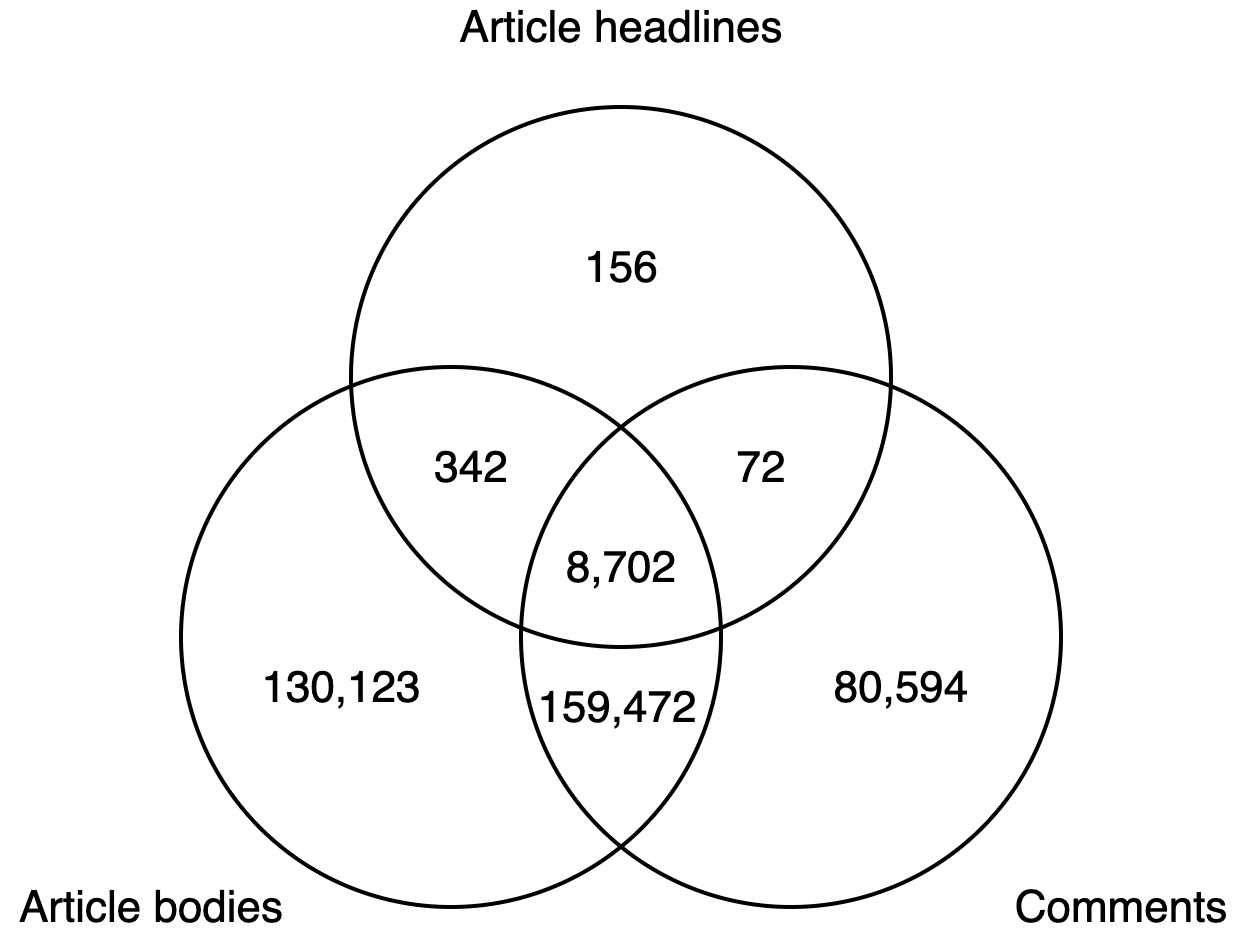
\includegraphics[scale=0.23]{0-img/vocab-venn-diagram.png}
    \caption{Venn diagram depicting overlap between each of the 3 domains in our Reddit dataset}
    \label{fig:vocab-venn-diagram}
\end{figure}